%
% Theory
%

% !TEX root = ../../main.tex

\chapter{Grundlagen}

\section{Natürliche Evolution vs. Artifical}

  Natürliche Evolution hat kein vordefiniertes Ziel und ist ein sogenannter open-ended Anpassungsprozess.
  Unter einem open-ended Anpassungsprozess in der natürlichen Evolution versteht man die Anpassung an die natürliche Umgebung.
  Da sich die natürliche Umgebung stetig ändert, ist der Prozess immer im Gange und endet nie.
  Artifizielle Evolution jedoch ist ein Optimierungsprozess,
  welcher versucht Lösungen zu vordefinierten Probleme zu finden~\cite[S.1]{book:bioInspired}.

  \subsection{Intelligent Design\label{sub:IntelligentDesign}}

    \todo[inline]{intelligent design}

\section{Artifical Evolution}

    \subsection{Individuum\label{sub:individual}}
      Als Individuum wird die zu evolvierende künstliche Kreatur bezeichnet.
      Ein Individuum hat einen zugehörigen Genotyp (\vref{sub:genotyp}) und dessen Phänotyp (\vref{sub:phenotyp}).
    \subsection{Genotyp\label{sub:genotyp}}
        Das genetische Material eines Individuums wird als Genotyp bezeichnet ~\cite[S.5]{book:bioInspired}.
        Es beeinhaltet alle wichtigen Informationen zur Reproduktion des Individuums.
        Das Genom ist eine Repräsentation des Genotyps.
    \subsection{Phänotyp\label{sub:phenotyp}}
        Der Genotyp kann zu einem Phänotyp abgebildet werden.
        In einer künstlichen Umgebung (wie der Pixelwelt des Computers) kann man sagen,
        dass der Phänotyp die Pixelrepräsentation des Genotyps ist.
        Wenn der Genotyp die Länge und Breite eines Rechtecks beschreibt, so ist das grafisch gezeichnete Rechteck auf dem Monitor der Phänotyp (\vref{fig:genoPheno}).
        \begin{figure}[H]
          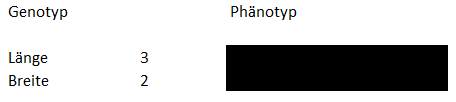
\includegraphics[scale=1]{graphics/genotyp_phenotyp}
          \caption{Genotyp und Phänotyp\label{fig:genoPheno}}
        \end{figure}

    %% in bioInspired wird genetic repärsentation erwähnt
    \subsection{Genetische Repräsentation}

    Der erste Schritt bei der Definition eines evolutionären Algorithmus ist die Auswahl der genetischen Repräsentation.
    Nicht alle Arten von evolutionären Algorithmen harmonieren mit jeder Repräsentation.
    Die genetische Repäsentation beschreibt die Elemente eines Genomes und wie diese in einen Phänotyp gemapped werden \cite[S.16]{book:bioInspired}.

      \subsubsection{Diskrete Repräsentation\label{par:GeneticRepresentationDiscrete}}

        Bei der diskreten Repräsentation wird das Genom als binären String dargestellt [0111110].
        Dieser binäre String kann anschliessend in einen Phänotyp übersetzt werden.
        Zum Beispiel kann eine Bitsequenz, direkt zu einer Zahl als Phänotyp übersetzt werden [0011] -> 3.
        Ebenfalls kann eine diskrete Repräsentation eine Folge von beliebigen Zeichen annehmen [ABCDEF].
        D. Floreano und C. Mattiussi bringen dazu ein gutes Beispiel anhand des Travelling Sales Man Problems an:
        Jeder Buchstabe in der Sequenz repräsentiert dabei einen Ort, welchen es zu besuchen gilt (\vref{fig:travelling}) \cite[S.18]{book:bioInspired}.

        \begin{figure}[H]
          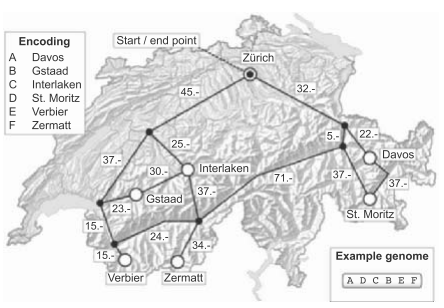
\includegraphics[scale=1]{graphics/discret_representation}
          \caption{Beispiel Diskrete Repräsentation \cite[S.18]{book:bioInspired} \label{fig:travelling}}
        \end{figure}

      \subsubsection{Reale-Werte-Repräsentation\label{par:GeneticRepresentationReal}}

        Weiter kann die Reale-Werte-Repräsentation gewählt werden.
        Das Genom wird hierbei durch reelle Zahlen repräsentiert.
        Beispielsweisse kann die optimale Position eines Zimmers (beste Flächennutzung) in einem Haus
        durch reale Zahlen dargestellt werden.

      \subsubsection{Baum-Repräsentationen\label{par:GeneticRepresentationTree}}

        Das zu evolvierende Objekt kann durch einen Baum dargestellt werden.
        \\
        Baum Repräsentationen (\vref{fig:baum}) werden eingesetzt um hierarchische Strukturen mit Verzweigungen und Bedingungen zu beschreiben ~\cite[S.19]{book:bioInspired}.
        Baumstrukturen haben den Vorteil, dass sie sehr gut rekursiv durchlaufen werden können. Viele Probleme aus der Informatik lassen sich einfacher rekursiv als iterativ lösen.
        \begin{figure}[H]
          \Tree[.* [.+ [.2 ] [.7 ] ].+ [.- [.5 ] [.1 ] ] ].*
          \caption{Darstellung einer Rechnung als Baum\label{fig:baum}}
        \end{figure}

    \subsection{Initiale Population}
      Die Grösse der zu evolvierenden Population kann selber bestimmt werden.
      Jedoch muss beachtet werden, dass eine grössere Population mehr Rechenaufwand bedeutet.
      Auch die Eigenschaften des Suchraums dürfen dabei nicht ignoriert werden.
      Wichtig bei der Erstellung einer initialen Population ist, möglichst diverse Individuen zu generieren,
      damit nicht wertvolle Lösungen verspielt werden.

    \subsection{Fitness-Funktion}

      Mit Hilfe der Fitness-Funktion lassen sich Individuen beurteilen,
      wie gut geeignet ihre Gene sind um die Problemstellung zu bewältigen.
      In der natürlichen Evolution ist die Fitness des Tieres, wie viele Nachkommen es erzeugen kann.
      In der technischen Welt jedoch muss der Anwender sie jeweils selber definieren und
      nach seiner Problemstellung anpassen. Oft ist die evaluation der Fitness-Funktion
      die rechenintensivste Teilaufgabe eines evolutionären Algorithmus ~\cite[S.22]{book:bioInspired}.

      %%%%%%%%%%%%%%%%%%%%%%%%%%%%%%%%%%%%%%%%%%%%%%%%%%%%%%%%%%%%%%%%%%%%%%%%%%%%%%%%%%%%%%%%%%%%%%%%%%%%%%%%%
      %%%%%%%%%%%%%%%%%%%%%%%%%%%%%%%%%%%%%%%%%%%%%%%%%%%%%%%%%%%%%%%%%%%%%%%%%%%%%%%%%%%%%%%%%%%%%%%%%%%%%%%%%
      %%%%%%%%%%%%!!!!!%%%%%%%%%%%%%%%%% BIS HIER KORIGIERT %%%%%%%%%%%%%%%%%%%%%%%%!!!!!%%%%%%%%%%%%%%%%%%%%%%
      %%%%%%%%%%%%%%%%%%%%%%%%%%%%%%%%%%%%%%%%%%%%%%%%%%%%%%%%%%%%%%%%%%%%%%%%%%%%%%%%%%%%%%%%%%%%%%%%%%%%%%%%%
      %%%%%%%%%%%%%%%%%%%%%%%%%%%%%%%%%%%%%%%%%%%%%%%%%%%%%%%%%%%%%%%%%%%%%%%%%%%%%%%%%%%%%%%%%%%%%%%%%%%%%%%%%

    \subsection{Selektionsoperation}

      Eine Selektionsoperation hilft einem möglichst gut geeignete Individuen einer Generation zu selektieren.
      Die Selektierten bilden die Basis für die nächste Generation.
      Eine grosse Herausforderung beim Selektieren ist die Erhaltung der Diversität.

      \subsubsection{Selektionsdruck}

        Als Selektionsdruck wird der Prozentsatz der Individuen der aktuellen Generation,
        welche man verwendet um Nachkommen zu erzeugen, bezeichnet.
        Dabei werden am nur die fittesten Individuen selektiert.
        Zum Beispiel bei 10 Individuen werden nur die 4 selektiert, welche den höchsten Fitnesswert aufweisen.
        Selektion nach Selektionsdruck hat den Nachteil, dass die Diversität schnell verloren geht.

      \subsubsection{Proportionale Selektion}

        Bei der proportionalen Selektion wählt man die Reproduktionsrate proportional zur Fitness.
        Proportionale Selektion funktioniert schlecht wenn alle Individuen sehr ähnliche Fitnesswerte aufweisen oder es nur wenige/einen Ausreisser gibt.

      \subsubsection{Rang-basierte Selektion}

        Es wird zuerst eine Rangliste erstellt und dann werden die Reproduktionswahrscheinlichkeiten proportional zum Rang zugeordnet.
        Diese Selektionsstrategy hat den Vorteil gegenüber der proportionalen Selektion,
        dass es nicht darauf ankommt wie unterschiedlich die Individuen sind.

      \subsubsection{Gekürzte Rang-basierte Selektion}

        Ähnlich wie die Rang-basierte Selektion.
        Es werden jedoch nur die besten Individuen zur Reproduktion selektiert und
        jedes Individuum produziert die gleiche Anzahl Nachkommen.

      \subsubsection{Turnier-basierte Selektion\label{par:Turnier}}

        Es werden \(k\) zufällig ausgewählte Individuen selektiert,
        das Individuum mit dem höchsten Fitnesswert erzeugt ein Nachkommen.
        Dies wird solange wiederholt bis man wieder so viele Nachkommen hat,
        wie die Ursprüngliche Generation Individuen hatte.
        Ein grosser Vorteil von Turniert-basierter Selektion ist die gute Balance zwischen
        Selektionsdruck und genetischer Diversität.

    \subsection{Rekombinationsfunktion}

        Bei der Rekombination werden jeweils Zwei Individuen selektiert und
        deren Gen-Paare werden rekombiniert (untereinander vertauscht).
        Rekombination ist nicht bei jeder Problemstellung hilfreich,
        es muss von Fall zu Fall neu bewertet werden ob sie eingesetzt wird.

        \subsubsection{One-Point Crossover}

          Es wird ein zufälliger Cross-Over Punkt bestimmt an dem die Gene des Paares vertauscht werden.
          Anwendbar ist diese Strategie bei Diskreten und Reale Werte Repräsentationen.

        \subsubsection{Multi-Point Crossover}

          Im Prinzip gleich wie One-Point Crossover, jedoch werden mehrere Punkte bestimmt und
          zwischen diesen Punkten werden dann die Gene ausgetauscht.

        \subsubsection{Uniform Crossover}

          Die Gene werden an \(n\) zufälligen Stellen vertauscht, nur Anwendbar auf Reale Werte Repräsentationen.

        \subsubsection{Arithmetic Crossover}

          Der Durschnitt von den Genen an \(n\) zufälligen Positionen wird gebildet.
          Aus diesem Durchschnitt wird dann ein Nachkomme erzeugt.
          Ebenfalls nur anwendbar auf Reale Werte Repräsentationen.

        \subsubsection{Sequenzen}

          Bei Sequenzen gilt es die Regel zu erhalten, dass alle Einträge nur einmal vorkommen dürfen.
          Wir erinnern uns an das Beispiel vom Travelling Sales Man~\vref{par:GeneticRepresentationDiscrete}.
          Es wird sozusagen eine Unique Version von  Multi-Point Crossover angewendet.

        \subsubsection{Bäume}

          Bei Bäumen wird ein zufälliger Teil des Baumes mit einem des anderen Nachkommens vertauscht.

    \subsection{Mutationsfunktion}

      Mutationen operieren direkt auf dem Individuum.
      Positionen eines Genoms werden mit einer bestimmten Wahrscheinlichkeit \(p_{m}\) mutiert.
      Es ist jedoch Vorsicht geboten, da gewisse Lösungen durch Mutationen verloren gehen können.

      \subsubsection{Binäre Repräsentationen}

        Wenn die Repräsentation aus binären Werten besteht, werden die Bits geflippt (oder nur bestimmte Segmente).

      \subsubsection{Reale Werte Repräsentationen}

        Es wird ein zufälliger Wert aus einer Gaus Verteilung \(N(0,\sigma)\) addiert.

      \subsubsection{Sequenzen}

        Zwei zufällig ausgewählte Positionen werden miteinander vertauscht.

      \subsubsection{Baum}

        Gewisse Teilabschnitte des Baumes werden mutiert.

    Genetische Repräsentation: Erbgutdaten, genetic encoding
    \\
    Phänotyp: Aussehen des Individuums -> Manifestation. In unserem Fall die 6-Beinigen Kreaturen als Pixelgrafik.
    \\
    Initialisieren -> Simulieren -> Selektion -> Rekombination -> Mutation -> Analyse
    \\
    Simulieren bis Analyse solange wiederholen bis zufrieden mit Resultat

  \subsection{Arten von evolutionären Algorithmen\label{sub:artenEvAlgos}}

    Es gibt insgesamt 4 Arten von evolutionären Algorithmen:
    Genetische Algorithmen, Genetische Programmierung, evolutionäre Programmierung
    und evolutionäre Strategien.

    \subsubsection{Genetische Algorithmen\label{item:genAlgo}}

      Die Genetischen Algorithmen arbeiten mit binären Genom Repräsentationen.
      Es wird sowohl Rekombination als auch Mutation eingesetzt.

    \subsubsection{Genetische Programmierung\label{item:genProg}}

      Es werden Bäume als Repräsentation des Genoms eingesetzt. Wie bei den Genetischen Algorithmen,
      wird auch Rekombination und Mutation eingesetzt.

    \subsubsection{Evolutionäre Programmierung\label{item:evProg}}

      Bei der evolutionären Programmierung wird ausschliesslich Mutation eingesetzt.
      Das Genom wird durch reale Werte repräsentiert. Als Selektionsoperator wird
      oft Turnier-basierte Selektion eingesetzt.

    \subsubsection{Evolutionäre Strategien\label{item:evStrat}}

        Ähnlich wie evolutionäre Programmierung, aber die Varianz der Verteilung,
        welche für die Mutation gebraucht wird ist genetische codiert.
